\chapter{Analysis}\label{sect:analysis}

\section{Fixed Points Analysis} \label{sect:fixed_point_analysis}

All of the models in the previous chapter represent discrete time mappings. As such, it is therefore possible to identify fixed points so as to better understand the behaviour of some of the models. As in~\cite{Hegselmann2002OpinionSimulation}, it is challenging to provide analytical insights for some combinations of these models. However, the Open model can be readily analysed with Passive listeners.


For a fixed point in this system, it must hold that $\underline{\underline{\mathbf{P}}}^{t+1} = \underline{\underline{\mathbf{P}}}^t$. This equation requires that no agent has updated its beliefs and so the system is unchanged. The structure of the method defined at the beginning of~\cref{sect:method} dictates that, at most, one listener agent will update at any one iteration. Hence, at most only one row of matrix $\underline{\underline{\mathbf{P}}}^t$ will change and so can be considered in isolation. 

Without loss of generality, let us select two agents from $\underline{\underline{\mathbf{P}}}^t$ and label them $\underline{\mathbf{P}}_s$ and $\underline{\mathbf{P}}_l$ respectively. Hence, for all agents, a fixed point must satisfy

\begin{equation}
    \underline{\mathbf{P}}_l = \alpha \cdot \underline{\mathbf{P}}_l + (1 - \alpha) \cdot \underline{\mathbf{P}}_s. \label{eq:open_FP}
\end{equation}

There are two possible ways this can occur. Firstly, when $\alpha = 1$, we have a trivial fixed point. Secondly, assuming $\alpha < 1$, the fixed point occurs when $\underline{\mathbf{P}}_l=\underline{\mathbf{P}}_s$ for all possible pairs of agents. This reveals that it is likely that a fixed point will be found when the agents have converged to a single shared belief, a claim that is supported in simulation. To test the stability of these fixed points, we take the eigenvalues of the Jacobian of \cref{eq:open_FP} which gives $\alpha \underline{\underline{\mathbf{I}}}$. The system is stable when the modulus of all of the eivenvalues lie within the unit circle. The trivial fixed point is clearly stable as $\abs{\alpha} = 1$. The non-trivial fixed point $\underline{\mathbf{P}}_l=\underline{\mathbf{P}}_s$ is asymptotically stable as $\abs{\alpha} < 1$. This shows that, under this particular scheme, the agents are guaranteed to cluster together, converging upon a consensus. However, the existence of a stable fixed point does not guarantee that the population converges to a belief with absolute certainty. 

Perhaps more interesting is the case of Bottom Up speakers and Passive listeners. Using the same notation as above, the equation to reveal fixed points becomes

\begin{equation}
    \underline{\mathbf{P}}_l = \alpha \cdot \underline{\mathbf{P}}_l + (1 - \alpha) \cdot \frac{\underline{\mathbf{A}} \odot \underline{\mathbf{P}}_l}{\underline{\mathbf{A}} \cdot \underline{\mathbf{P}}_l}. \label{eq:BU_FP}
\end{equation}

From this equation, it can be shown that there are three fixed points. The first is trivial at $\alpha = 1$. The second occurs when $P_L(\mathbf{A}) = 0$ meaning that the listener has a $0$ probability for every state that the speaker has asserted and so does not update. The third occurs when $P_L(\mathbf{A}) = 1$, meaning that the speaker has asserted at least every state for which the listener has a non-zero probability. This final fixed point indicates that

\begin{align*}
    \underline{\mathbf{P}}_l = \frac{\underline{\mathbf{A}} \odot \underline{\mathbf{P}}_l}{\underline{\mathbf{A}} \cdot \underline{\mathbf{P}}_l}.
\end{align*}

This condition highlights two things: firstly, that $ \underline{\mathbf{A}} \cdot \underline{\mathbf{P}}_l = 1 $; secondly, that $ \underline{\mathbf{A}} \odot \underline{\mathbf{P}}_l =  \underline{\mathbf{P}}_l$. These are equivalent to $\sum^n_j A_j p_{l,j} = 1$ and $ p_{l,j} = A_j p_{l,j} $ respectively. 

As previously, to show the stability of these fixed points, the Jacobian must be computed. First, consider the diagonal elements of $\underline{\underline{\mathbf{J}}}$, given by

\begin{align}
    J_{a,a} = \frac{d f(p_{l,a})}{d p_{l,a}} &= \frac{d}{d p_{l,a}} \left( \alpha p_{l,a} + (1 - \alpha) \cdot \frac{A_a p_{l,a}}{\sum^n_j A_j p_{l,j}} \right) \\
    &= \alpha + (1 - \alpha) \cdot \left( \frac{A_a}{\sum^n_j A_j p_{l,j}} - \frac{A_a^2 p_{l,a}}{\sum^n_j A_j p_{l,j}} \right) \\
    &= \alpha + (1 - \alpha) \cdot \frac{A_a}{\sum^n_j A_j p_{l,j}} \left( 1 - \frac{A_a p_{l,a}}{\sum^n_j A_j p_{l,j}} \right), \\ 
\end{align}

and off-diagonals are given by

\begin{align}
    J_{a,b} = \frac{d f(p_{l,a})}{d p_{l,b}} &= \frac{d}{d p_{l,b}} \left( \alpha p_{l,a} + (1 - \alpha) \cdot \frac{A_a p_{l,a}}{\sum^n_j A_j p_{l,j}} \right) \\
    &= 0 + (1 - \alpha) \cdot \left( - \frac{A_a p_{l,a} A_b}{\sum^n_j A_j p_{l,j}} \right). \\
\end{align}


When $\alpha = 1$, it can be seen that off-diagonals are $0$, and the diagonal elements are $1$, therefore the eigenvalues of $\underline{\underline{\mathbf{J}}}$ are $1$. When $P_L(\mathbf{A}) = 0$, the diagonal elements of $\underline{\underline{\mathbf{J}}}$ are $\alpha$, however, the off-diagonals are not so clear. Consider the full $n \times n$ real matrix

\begin{center}
$\underline{\underline{\mathbf{J}}} = \begin{bmatrix}
    \alpha - (1 - \alpha) A_1 (1- p_{l,1}) & - (1 - \alpha) A_1 p_{l,2} & \dots  & -(1 - \alpha) A_1 p_{l,n} \\
    - (1 - \alpha) A_2 p_{l,1} &  \alpha - (1 - \alpha) A_2 (1- p_{l,2}) &  \dots  & -(1 - \alpha) A_2 p_{l,n} \\
    \vdots & \vdots & \ddots & \vdots \\
    - (1 - \alpha) A_n p_{l,1} & - (1 - \alpha ) A_n p_{l,2} &  \dots & \alpha - (1 - \alpha) A_n (1- p_{l,n}) \\

\end{bmatrix}$.
\end{center}

For stability, the modulus of the eigenvalues of this matrix must lie within the unit circle, however, it is not possible to evaluate each eigenvalue in the general case for $n>5$, due to the Abel-Ruffini Theorem~\cite{Abel1824MemoireDegre}. With some minor manipulations to this matrix, it is possible to apply Perrón-Frobenius theorem to calculate the largest positive real eigenvalue, but this is insufficient for determining the stability, as there is no guarantee that all the eigenvalues are real~\cite{Perron1907ZurMatrices}. Fortunately, Gershgorin Circle Theorem provides a method for bounding the location of the eigenvalues in the complex plane~\cite{Gerschgorin1931UberMatrix}. This theorem states that each eigenvalue $\lambda_a$ of an $n\times n$ square matrix $\underline{\underline{\mathbf{M}}}$ will lie within at least one Gershgorin Disc $D(m_{a,a}, R_a)$ where the centre of the disc $m_{a,a}$ is the $a^\textnormal{th}$ element on the diagonal of $\underline{\underline{\mathbf{M}}}$, and its radius $R_a = \sum^n_{b \neq a}\abs{m_{a,b}}$. Consider \cref{fig:gershgorin}. This figure shows the unit circle in the complex plane and three Gershgorin Discs. If all of the discs were within the unit circle, our system would be stable. It should be noted that, because the eigenvalues must lie within at least one of these discs, having a disc outside the unit circle is a necessary but not sufficient condition for determining that the system is unstable. \\


\begin{figure}
\begin{center}
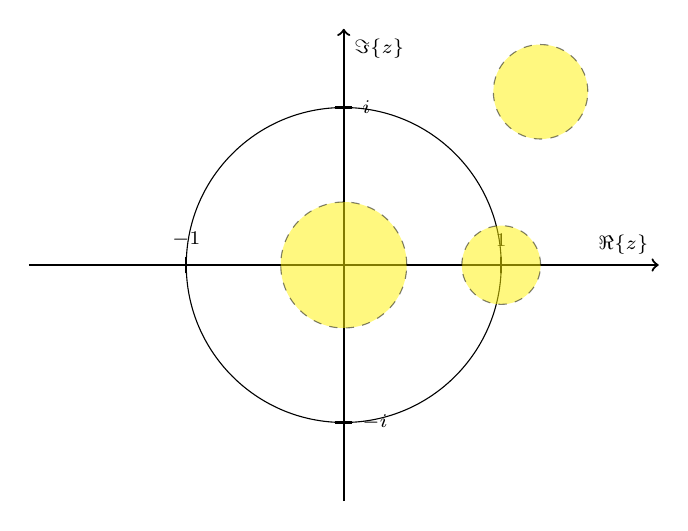
\begin{tikzpicture}
     \begin{scope}[thick,font=\scriptsize]
     % Axes:
     % Are simply drawn using line with the `->` option to make them arrows:
     % The main labels of the axes can be places using `node`s:
     \draw [->] (-4,0) -- (4,0) node [above left]  {$\Re\{z\}$};
     \draw [->] (0,-3) -- (0,3) node [below right] {$\Im\{z\}$};
 
     % Axes labels:
     % Are drawn using small lines and labeled with `node`s. The placement can be set using options
     \iftrue% Single
     % If you only want a single label per axis side:
     \draw (2,-3pt) -- (2,3pt)   node [above] {$1$};
     \draw (-2,-3pt) -- (-2,3pt) node [above] {$-1$};
     \draw (-3pt,2) -- (3pt,2)   node [right] {$i$};
     \draw (-3pt,-2) -- (3pt,-2) node [right] {$-i$};
     \else% Multiple
     % If you want labels at every unit step:
     \foreach \n in {-4,...,-1,1,2,...,4}{%
         \draw (\n,-3pt) -- (\n,3pt)   node [above] {$\n$};
         \draw (-3pt,\n) -- (3pt,\n)   node [right] {$\n i$};
     }
     \fi
     \end{scope}
     % The circle is drawn with `(x,y) circle (radius)`
     % You can draw the outer border and fill the inner area differently.
     % Here I use gray, semitransparent filling to not cover the axes below the circle
     \path [draw=black] (0,0) circle (2);
     \path [draw=black, dashed, fill=yellow, semitransparent] (0,-0) circle (0.8);
     \path [draw=black, dashed, fill=yellow, semitransparent] (2,0) circle (0.5);
     \path [draw=black, dashed, fill=yellow, semitransparent] (2.5,2.2) circle (0.6);
     % Place the equation into the circle:
\end{tikzpicture}
\end{center}
\caption{A plot of an Argand diagram demonstrating Gershgorin Circle Theorem. The system is stable if the eigenvalues are all within the unit circle, shown in black. The yellow circles show Gershgorin discs of a system. The theorem dictates that each eigenvalue must lie within at least one of these discs. }
\label{fig:gershgorin}
\end{figure}

Therefore, for the fixed point $P_L(\mathbf{A}) = 0$, the eigenvalues lie within Gershgorin Discs of the form 

\begin{align}
    &D(\alpha, \sum_{b \neq a}^n \abs{ - (1 - \alpha) A_a p_{l,b} } ) \nonumber \\
    &D(\alpha, \sum_{b \neq a}^n (1 - \alpha) A_a p_{l,b} ) \nonumber \\
    &D(\alpha, (1 - \alpha) A_a (1 - p_{l,a}) ) .
\end{align}

Here, as $\underline{\mathbf{A}}$ is a binary vector, this equation can be broken down into two cases. Firstly, let $A_a = 0$. In this case, the disc becomes $D(\alpha, 0)$, which is within the unit circle. Secondly, let $A_a = 1$. In this case, $p_{l,a} = 0$, and therefore the disc becomes $D(\alpha, 1-\alpha)$, which makes contact with, but does not cross, the unit circle. Hence, for $P_L(\mathbf{A}) = 0$, the fixed point is stable. 

A similar argument exists for the fixed point at $P_L(\mathbf{A}) = 1$. Here, the eigenvalues of $\underline{\underline{\mathbf{J}}}$ must lie within discs of the form 

\begin{align}
 D(\alpha - ( 1 - \alpha ) A_a ( 1 - p_{l,a}), \sum_{b \neq a}^n \abs{ - (1 - \alpha) A_a p_{l,b} }) \nonumber\\
 D( \alpha - (1 - \alpha) A_a (1 - p_a), (1 - \alpha) A_a (1 - p_{l,a})).  
\end{align} \label{eq:2FPGershgorin}

As $\underline{\mathbf{A}}$ is a binary vector, we can split~\cref{eq:2FPGershgorin} into two different types of disc, one in which $A_a = 0$ and one in which $A_a = 1$. When $A_a = 0$, the discs are $D(\alpha, 0)$, and so are within the unit circle. When $A_a = 1$, the discs are given by \[ D(\alpha + (1 - \alpha) (1 - p_{l,a}), (1 - \alpha)(1 - p_{l,a})).\] Therefore, the system is stable when \[ \alpha + 2(1 - \alpha)(1 - p_{l,a}) \leq 1.   \]

This simplifies to 
\begin{align}
    \alpha + 2(1 - \alpha) ( 1- p_{l,a}) & \leq 1 \nonumber  \\
    2(1 - \alpha - p_{l,i} + \alpha p_{l,i}) & \leq 1 - \alpha \nonumber\\
    - 2p_{l,a} + 2\alpha p_{l,a} & \leq \alpha - 1 \nonumber \\
    2 p_{l,a} (\alpha - 1) & \leq \alpha - 1 \nonumber \\
    p_{l,a}  & \geq \frac{1}{2}.
\end{align}

Hence, when $A_a = 0$, each corresponding disc is within the unit circle and when $A_a = 1$, the system as a whole is guaranteed to be stable when $p_{l,a} \geq \frac{1}{2}$. This can only happen in one of two ways: $p_{l,a} = 1$ and all other probabilities are $0$, or there are two states for which $p_{l,a} = \frac{1}{2}$. Therefore, it is expected that the system will tend to steady states in which, for every agent, either $p_{l,a} = 1 \textnormal{ or } p_{l,a} = \frac{1}{2}$. Therefore, it is expected that the agents will graduate toward either certainty in a single state of the world or equal levels of uncertainty in two states. 





\section{Simulation Experiments}

The following experiments were run on an Intel(R) Core i7-8650 CPU 1.90Ghz with the following parameters as default, unless otherwise stated: $n=3, K=100, \alpha = 0.3, \gamma = 0.5, t_{max} = 50,000, \eta = 10^{-5}, T=3$. Error bars are shown at $\pm \sigma$, one standard deviation. 
\subsection{Consensus}

To gain an insight into the dynamics of these systems, let us consider their entropy, as defined in~\cref{eq:shannon_entropy}. This serves as a measure of the uncertainty in the system. High values imply the absence of strong beliefs in the population, and low values imply a level of certainty, though importantly, not consensus. To illustrate the distinction between these entropy values, consider \cref{fig:2d-simplex}. There are some agents in the corners of the Barycenter plot that are initialised with strong beliefs in one states of the world. These agents will have low entropy values, whereas those closer to the centre of the plot will have much higher entropy values due to their uncertainty. 


\Cref{fig:entropy_all,fig:J-div_all} show plots of entropy and J-Divergence changing over time for each of the four models proposed. Here, the listeners are Passive. In can be seen that the entropy and the J-Divergence of the Open model follow significantly different trajectories to the other models. The J-Divergence decreases, as in the other models, although it reaches $0$ almost immediately. This suggests that the agents cluster together rapidly. The entropy plot, however, differs significantly to the other models. It can be seen to increase to a value of $\approx 1.09$. This is approximately the maximum entropy value that could be obtained in a $3$-dimensional world. It is apparent that the agents quickly cluster together, each of them assuming the uniform distribution as their beliefs. This is due to their uniformly random initialisation, not a characteristic of the model. Therefore, the Open model behaves as predicted by~\cref{sect:fixed_point_analysis}, converging to a single point that is approximately the average of every agent's beliefs. It should be noted that there is limited variation in the behaviour of the Open model, as evidenced by the narrow error bars. 

\begin{figure}[H]
 \centering
  \begin{minipage}[ht]{0.49\textwidth}
    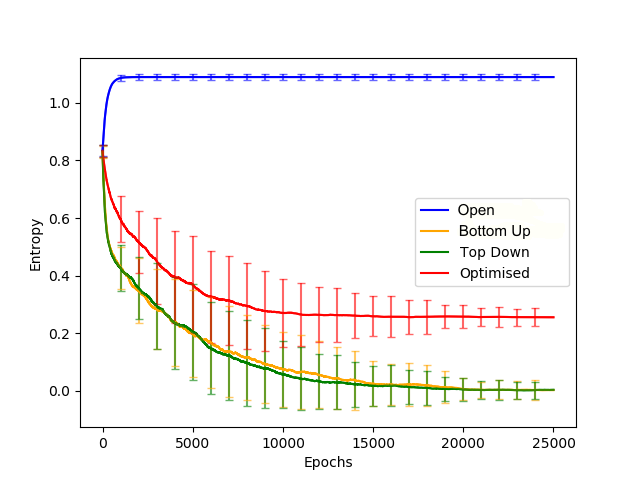
\includegraphics[width=\textwidth]{Images/Figures/All/Entropy_25000.png}
    \subcaption{Entropy}\label{fig:entropy_all}
 \end{minipage}
 \hfill
 \begin{minipage}[ht]{0.49\textwidth}
    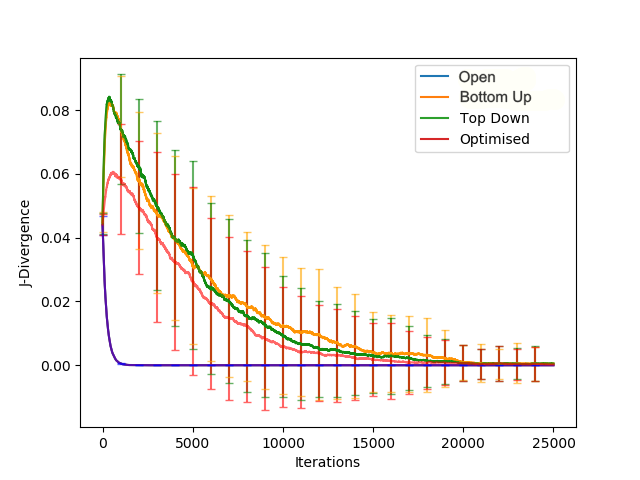
\includegraphics[width=\textwidth]{Images/Figures/All/J-Div_25000.png}
    \subcaption{J-Divergence}\label{fig:J-div_all}
 \end{minipage}
 \caption{Two plots to show the change in entropy and J-Divergence over time, for the Open, Bottom Up, Top Down, and Optimised models. These plots were obtained using Passive listeners, and were averaged over $100$ runs.}
\end{figure}

The Bottom Up and Top Down models seem to behave indistinguishably, both reducing the uncertainty in the population as time passes, tending toward $0$ at a similar rate for both entropy and J-Divergence. These two approaches are capable of achieving a population of agents that are certain of one state alone. In order to determine whether one is a dominant strategy, the two models must be compared across a variety of different parameter values, explored in the following section.  It should be noted that all models other than the Open model appear to \emph{increase} the disagreement between agents for the first few hundred iterations. This occurs at the same time as the gradient of the entropy plot is maximal. At this time, agents are quickly persuaded toward one particular state, depending on the arguments they hear. Due to the random initialisation, this divides the population, increasing the J-Divergence until a majority forms in support of one possible state and the agents begin to converge toward it. In simulation, this phenomenon manifests in some interesting patterns such as those shown in~\cref{fig:sierpinski_triangle_intro}. 


\begin{figure}[H]
    \centering
    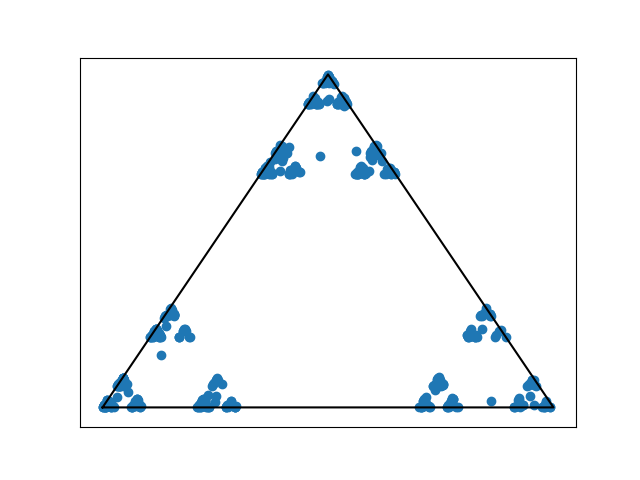
\includegraphics[width=0.45\textwidth]{Images/Figures/Barycenter/Serpinski_example.png}
    \caption{The $500^\textnormal{th}$ iteration of a simulation of the Bottom Up model. $500$ agents are shown, with clusters of agents forming at $\underline{\mathbf{P}}^t_{x} \approx [\alpha, 1-\alpha, 0]^T$. The listeners are Passive. Importantly, the system has not converged at this point.}
    \label{fig:sierpinski_triangle_intro}
\end{figure}

When a listener that has a strong belief in $H_j$ is presented with an assertion $ \mathbf{A} = \{ H_{¬j} \}$, approximately the following update occurs. 


\begin{center}
$\underline{\mathbf{P}}^t_l = \alpha \begin{bmatrix}
    1-\epsilon\\
    \epsilon\\
    0
\end{bmatrix} + (1 - \alpha) \frac{\begin{bmatrix} 0\\1\\0 \end{bmatrix} \odot \begin{bmatrix} 1-\epsilon\\ \epsilon\\ 0 \end{bmatrix}} {\begin{bmatrix} 0\\1\\0 \end{bmatrix} \cdot \begin{bmatrix} 1- \epsilon\\ \epsilon \\ 0\end{bmatrix}} $, \\
\end{center}
where $\epsilon$ is an arbitrarily small positive number, such that $\sum^n_j p^t_{l,j} = 1$. Then 
\begin{center}
$\underline{\mathbf{P}}^t_l =\alpha \begin{bmatrix}
    1 - \epsilon \\
    \epsilon\\
    0
\end{bmatrix} + (1 - \alpha) \begin{bmatrix} 0\\ 1 \\ 0  \end{bmatrix} $ \\

$\underline{\mathbf{P}}^t_l \approx \begin{bmatrix} \alpha \\ 1 - \alpha \\ 0  \end{bmatrix}$.
\end{center}

As an aside, when $\alpha = 0.5$, the plot shows remarkable similarity to the Sierpinski Triangle due to the same phenomenon as~\cref{fig:sierpinski_triangle_intro}, demonstrated in~\cref{fig:sierpinski_compare}. 

\begin{figure}[H]
  \begin{minipage}[t]{0.49\textwidth}
    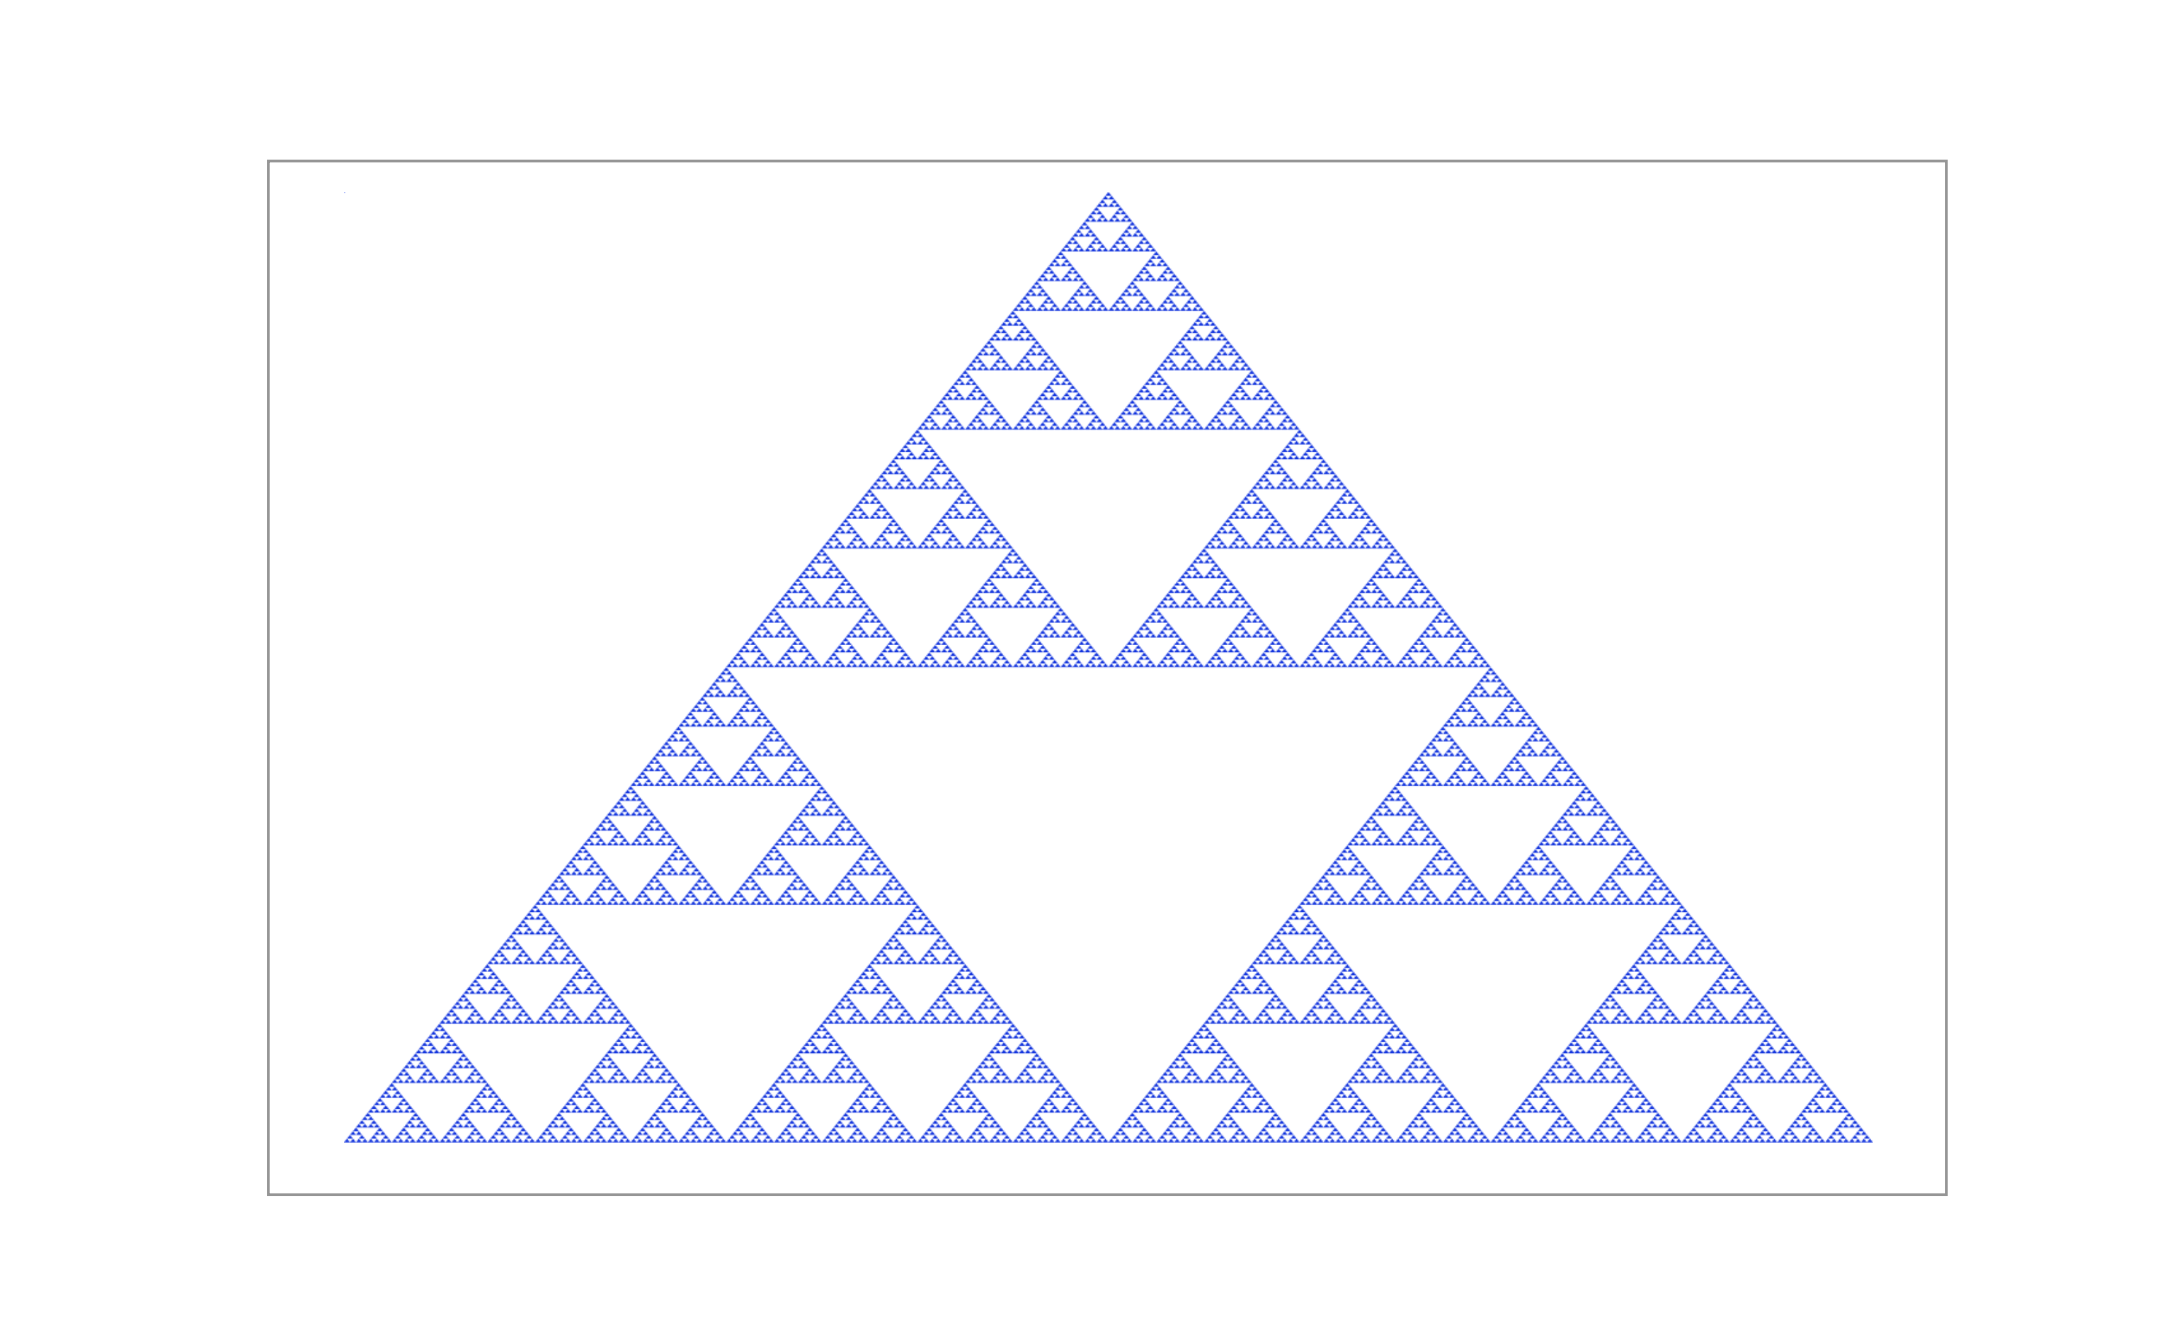
\includegraphics[width=\textwidth]{Images/Misc/Sierpinski_triangle_real_resized.png}
    \subcaption{Sierpinski Triangle}
  \end{minipage}
  \hfill
 \begin{minipage}[t]{0.49\textwidth}
    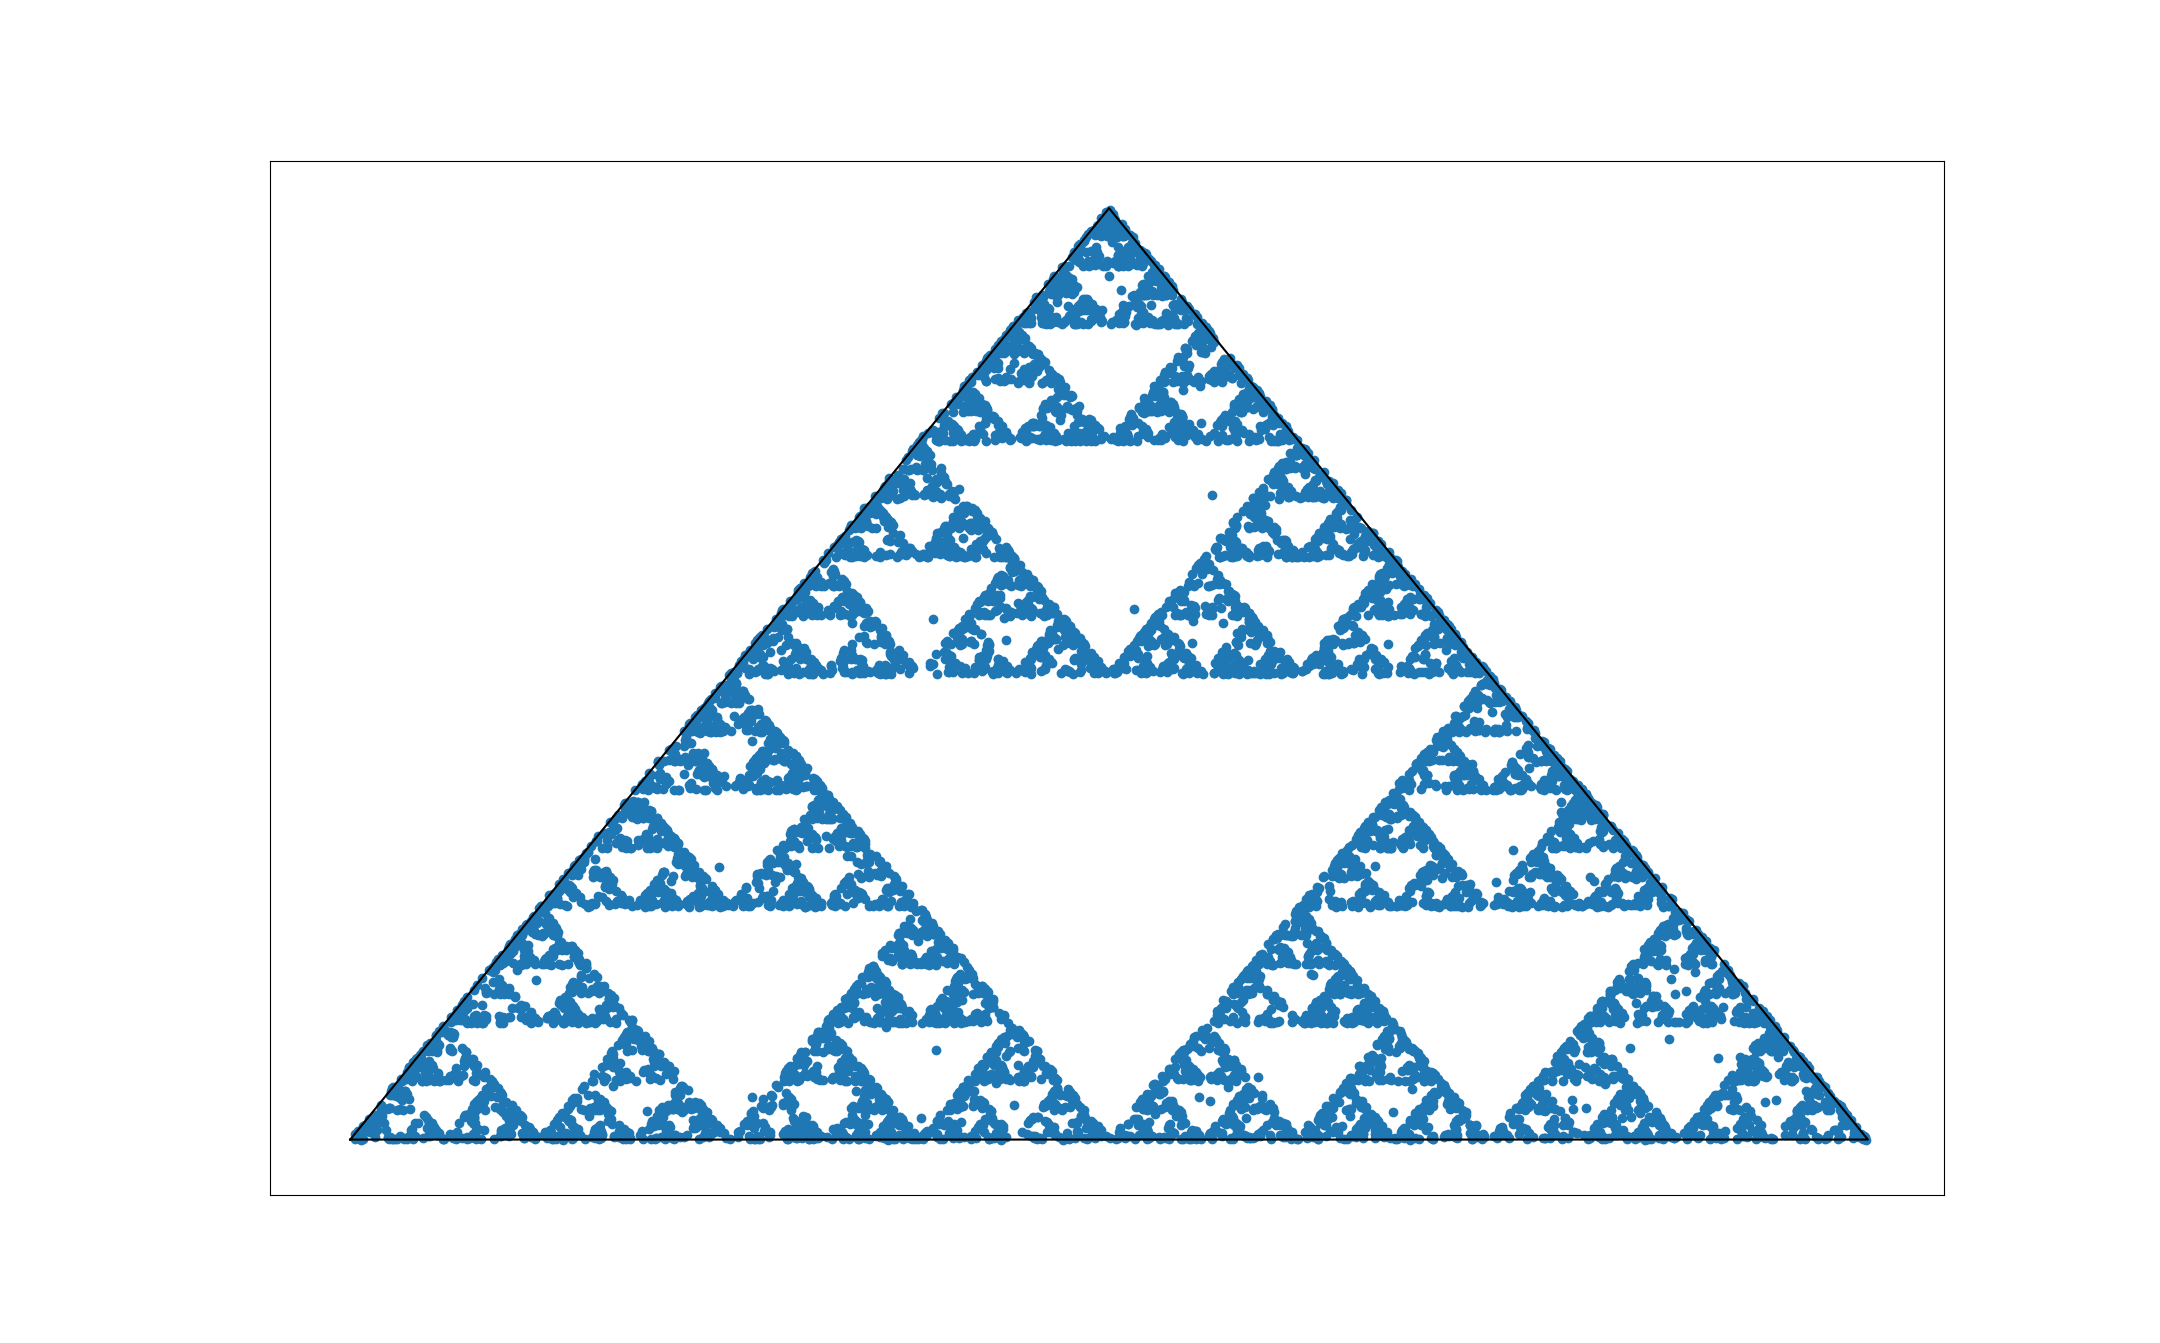
\includegraphics[width=\textwidth]{Images/Figures/Barycenter/Serpinski_BU.png}
    \subcaption{Bottom Up Model} \label{fig:sierpinski_BU}
 \end{minipage}
 \caption{ The true Sierpinski Triangle, and the Bottom Up model after $80,000$ iterations with $K=10,000, \alpha=0.5$. The pattern in (b) is not stable and breaks down with time. \\ \textit{Image downloaded from \url{https://bit.ly/2GkoUXI}}  }\label{fig:sierpinski_compare}
\end{figure}


The population in the Bottom Up model forms a particular structure, as shown in~\cref{fig:sierpinski_BU}. The explanation for this structure arises due to the similarity between the update rule and a chaos game. Originally described by Barnsley, a chaos game
\begin{displayquote} 
    ``\dots is a Markov Chain Monte Carlo algorithm that is applied in order to describe probability distributions supported on an attractor of an iterated function system''~\cite{Barnsley2011ChaosSpaces}.
\end{displayquote}

To better understand them, an example of a chaos game is taken from \cite{Feldman.DavidP2012ChaosIntroduction} that bears a resemblance to the general speaker-listener model described in~\cref{sect:method}. In his book, Feldman begins by selecting a point anywhere within the outermost triangle shown in \cref{fig:chaos_game}. Then, if such a device were practical, a three-sided die is rolled, and the point is moved half-way toward the result of the roll. For example, let the first die roll be a $2$. The point would then move to be within the upper shaded triangle, labelled ``$2$''. If the subsequent roll was a $3$, then the point would lie anywhere within the triangle, marked ``$2,3$''. This process can be repeated ad infinitum creating infinitely dense trajectories of this point, as well as revealing areas that it is impossible for the point to reach, shown in white. After an infinite number of iterations, the trajectory of this point will reveal the Sierpinski triangle. Similar results are obtained using the update rule for Passive listeners in which agents update their beliefs toward a vertex that, at least in the early stages of the population's communications, is chosen almost uniformly at random. However, as soon as a large cluster of agents forms, the balance of probability shifts toward them, so the fractal structure of the population begins to break down. In the Optimised model, occasionally the largest cluster can form at a vertex of one of the sub-triangles and remain there, as shown in~\cref{fig:optimised_problem_case}. A further difference is that Passive listeners update toward the vertex by some function $f(\alpha)$, instead of the point moving half-way toward the selected vertex.  

\begin{figure}[]
\begin{center}
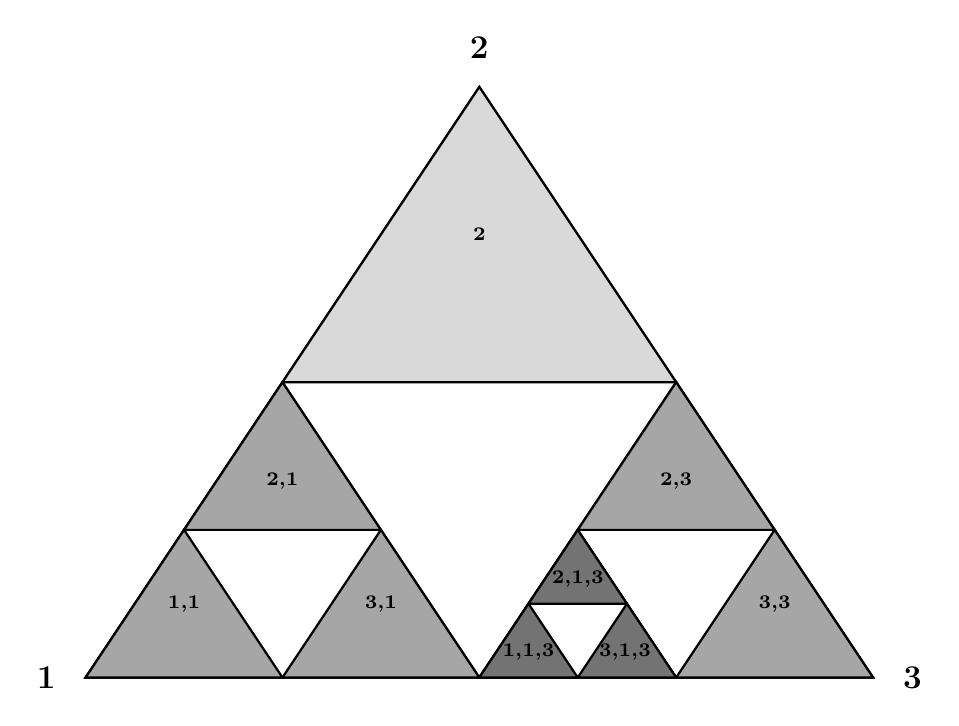
\begin{tikzpicture}
    \draw[thick] (0,0) -- (10,0) -- (5,7.5) -- cycle;
    
    \draw[thick] (0,0) -- (5,0) -- (2.5,3.75) -- cycle;  
    \draw[thick] (10,0) -- (5,0) -- (7.5,3.75) -- cycle;
    \draw[thick, fill=black!15] (2.5,3.75) -- (7.5,3.75) -- (5,7.5) -- cycle;

    
    \draw[thick, fill=black!35] (0,0) -- (2.5,0) -- (1.25,1.875) -- cycle;
    \draw[thick, fill=black!35] (2.5,0) -- (5,0) -- (3.75,1.875) -- cycle;
    \draw[thick, fill=black!35] (1.25,1.875) -- (3.75,1.875) -- (2.5,3.75) -- cycle;
    \draw[thick] (5,0) -- (7.5,0) -- (6.25,1.875) -- cycle;
    \draw[thick, fill=black!35] (7.5,0) -- (10,0) -- (8.75,1.875) -- cycle;
    \draw[thick, fill=black!35] (6.25,1.875) -- (8.75,1.875) -- (7.5,3.75) -- cycle;
    
    
    \draw[thick, fill=black!55] (5,0) -- (6.25,0) -- (5.625,0.9375) -- cycle;
    \draw[thick, fill=black!55] (6.25,0) -- (7.5,0) -- (6.875,0.9375) -- cycle;
    \draw[thick, fill=black!55] (5.625,0.9375) -- (6.875,0.9375) -- (6.25,1.875) -- cycle;

    \node at (5,5.625) {\scriptsize\textbf{2}};
    \node at (5,8) {\large\textbf{2}};
    \node at (-0.5,0) {\large\textbf{1}};
    \node at (10.5,0) {\large\textbf{3}};
    
    \node at (1.25,0.9375) {\scriptsize\textbf{1,1}};
    \node at (2.5, 2.5) {\scriptsize\textbf{2,1}};
    \node at (3.75, 0.9325) {\scriptsize\textbf{3,1}};
    
    \node at (7.5, 2.5) {\scriptsize\textbf{2,3}};
    \node at (8.75, 0.9325) {\scriptsize\textbf{3,3}};
    
    \node at (5.625, 0.32625) {\scriptsize\textbf{1,1,3}};
    \node at (6.25, 1.25) {\scriptsize\textbf{2,1,3}};
    \node at (6.85, 0.32625) {\scriptsize\textbf{3,1,3}};

\end{tikzpicture}
\end{center}
\caption{A pictorial representation of a chaos game to generate a Sierpinski Triangle. A point is chosen at random from the outermost triangle then, at each iteration, is updated half-way toward a randomly selected vertex. The triangle marked ``$3,1,3$'' represents the area that the randomly selected first point must be in if the sequence of vertices has been first $3$, then $1$ then $3$. Repeated ad infinitum, this process will generate a Sierpinski Triangle.}  \label{fig:chaos_game}
\end{figure}

Finally, the Optimised model appears to be failing to live up to its name. While it does induce a reduction in the entropy of the system, it does not enable the agents to become certain that any one state is true. That said, the agents do arrive at a consensus, as evidenced by the J-Divergence plot. This indicates that the agents converge to a single point in probability space, but that that point is not in a corner of the Barycenter plot, and thus the agents are not certain in a single state. \Cref{fig:optimised_problem_case} shows a histogram of the final states of agents using the Optimised approach. 

\begin{figure}[]
    \centering
    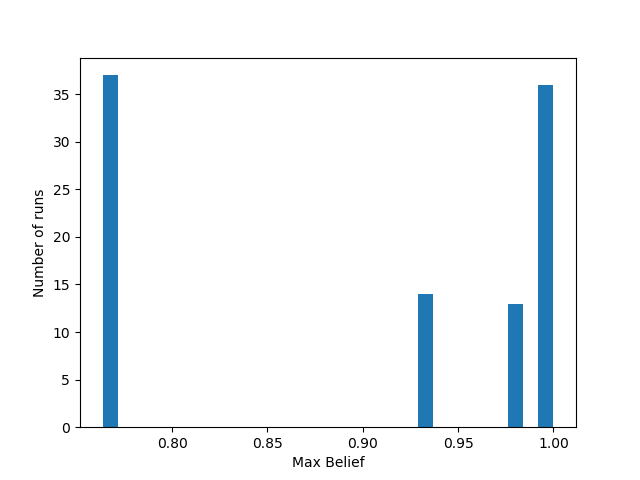
\includegraphics[width=0.59\textwidth]{Images/Figures/Optimised/ChaoticAttractorMaybe.png}
    \caption{ A histogram showing the maximum probability at the $25,000^\textnormal{th}$ iteration of the Optimised model, for $100$ runs. It can be seen that there are two main locations the agents converge to, with other, less frequent possibilities in between.  }
    \label{fig:optimised_problem_case}
\end{figure}

\Cref{fig:optimised_problem_case} shows a histogram of $100$ runs at $\alpha =0.3$, with the maximum probability of the agents at steady state on the $x$-axis. It can be seen that the maximum probability values are not random, instead, clustering together at particular values, approximately $0.76, 0.93, 0.98$ and $1$. The differences between these values consecutively can be approximated to $\frac{1}{3}$ multiplied by the difference between the previous pair of probabilities. This ratio is $\approx \alpha$, suggesting that the Optimised model does not always converge to a vertex of the Barycenter plot, instead converging to a vertex of one of the sub-triangles shown in~\cref{fig:chaos_game}. 

In order to better understand why this happens, we must return to the objective function of this model. Since the speaker seeks to minimise the J-Divergence between itself and the listener, at this final state, the speaker has two options. If it were to assert the single most probable state, the listener would likely become more certain in that single state, gradually allowing the population to become certain in a single state of the world. However, if the speaker were to assert that singleton, the J-Divergence between the speaker and listener would clearly increase, so it is optimal for the speaker to assert something that does not cause the listener to move away, even if this were to improve the collective certainty. From this analysis, it is clear that the Optimised model is, in fact, sub-optimal, showing that unconstrained speakers are detrimental to the decision-making abilities of the group. 



\subsection{Convergence}

In order to compare the behaviour of the Bottom Up and Top Down models, let us examine their convergence across the variation of $\gamma$ between $0$ and $1$. The Open and Optimised models are unaffected by $\gamma$ and so have not been included. Recall that the system is said to have converged if $\Delta \hat{E}^{T+t} = \abs{ \hat{E}^t -  \hat{E}^{t+T}}  \leq \eta$. \Cref{fig:convergence_none} shows the results. 

\begin{figure}[h!]
 \centering
  \begin{subfigure}[ht]{0.45\textwidth}
    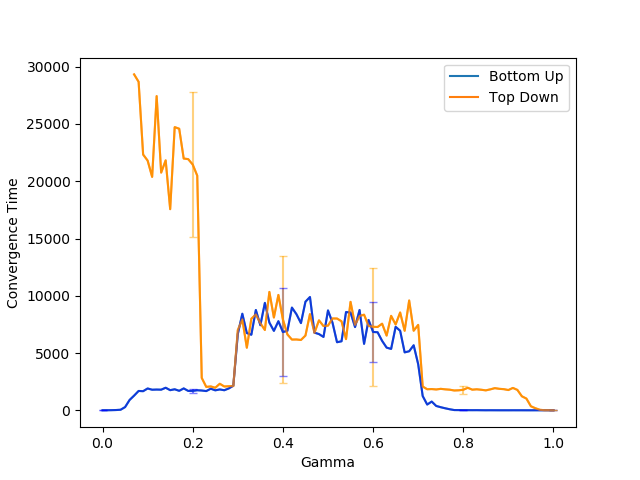
\includegraphics[width=\textwidth]{Images/Figures/BU+TD/None/Convergence_best.png}
    \caption{Convergence}\label{fig:convergence}
 \end{subfigure}
 \hfill
 \begin{subfigure}[ht]{0.45\textwidth}
    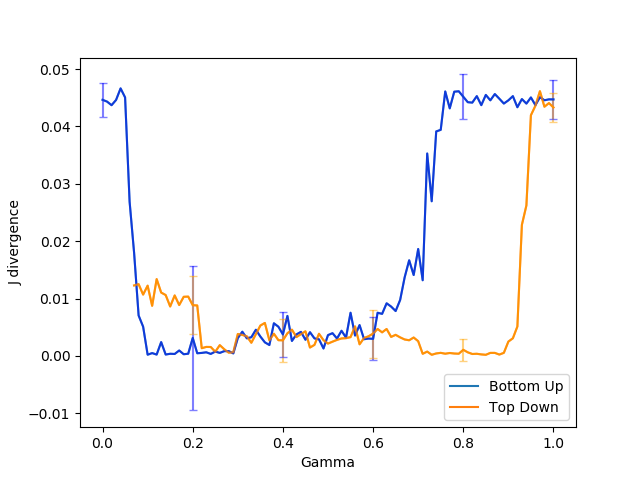
\includegraphics[width=\textwidth]{Images/Figures/BU+TD/None/J-Div_best.png}
    \caption{J-Divergence}\label{fig:J-Div_convergence}
 \end{subfigure}
 \hfill
 \begin{subfigure}[ht]{0.45\textwidth}
    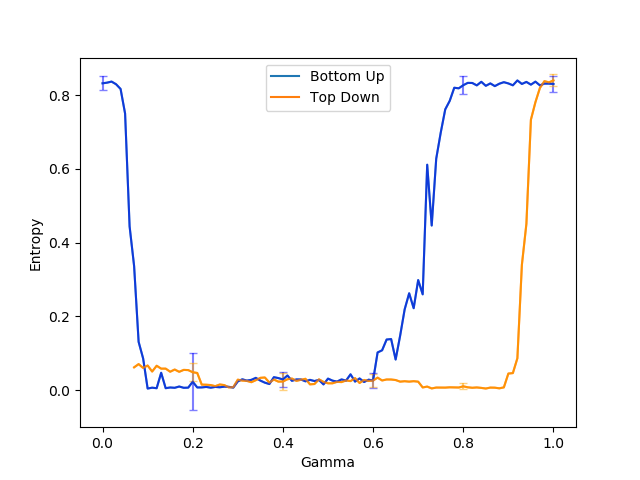
\includegraphics[width=\textwidth]{Images/Figures/BU+TD/None/Entropy_best.png}
    \caption{Entropy}\label{fig:entropy_convergence}
 \end{subfigure}
 \caption{ Three plots showing the convergent behaviour of the Bottom Up and Top Down models with Passive listeners as $\gamma$ is varied. (a) shows the time to convergence as defined by~\cref{eq:convergence}. (b) shows the average J-Divergence of the system at the corresponding iteration of (a). (c) shows the average entropy of the system at the corresponding iteration of (a). If the system has not converged within $50,000$ iterations, the point is left blank. }\label{fig:convergence_none}
\end{figure}

It is apparent that, for both models, high values of $\gamma$ relate to very rapid convergence. This can be attributed to the fact that at values of $\gamma \approx 1$, it is impossible for either model to create a meaningful assertion; they are limited to asserting $\emptyset$ in the Bottom Up model and $\mathbf{W}$ in the Top Down. Neither of these assertions produces any change in the listener. This registers as rapid convergence as the entropy remains constant coinciding with the increases in entropy and J-Divergence for $\gamma > 0.8$.

In the Bottom Up plots, one can observe rapid convergence for values of $\gamma \geq 0.6$. At this point, it is impossible for the speaker to assert anything other than a singleton, meaning that its arguments are guaranteed to be precise. This phenomenon increases the rate of convergence. Furthermore, as $\gamma$ increases, the only agents that can put forward any non-trivial argument are those who already hold extreme beliefs with high probability in one particular state. This accelerates the movement of the general population toward the region in which only extremist speakers can speak until more and more of the population holds similarly strong beliefs. This effect accelerates as more agents become able to assert something. 

It is also possible to observe a sharp increase in convergence time shortly after $ \gamma = \frac{1}{n}$. As $\gamma$ increases above this point, it begins to create a region of probability space in which it is impossible for an agent to assert anything, making them purely passive. For instance, if $\mathbf{P}_S =\{ 0.3, 0.3, 0.4\}$ and $\gamma = 0.5$, it is impossible for the speaker to assert anything. This will increase the convergence time as, if such an agent is picked, it is incapable of asserting anything meaningful. Meanwhile, the agents that can speak are likely to be asserting slightly general statements so convergence is slow until $\gamma$ approaches $0.6$. In the region $0.3 \leq \gamma \leq 0.6$, it can be seen that both models behave similarly, both converging within $7,500$ iterations. 

The Top Down approach exhibits some different behaviour with slow convergence times for low values of $\gamma$. The slow convergence for low $\gamma$ is attributable to oscillations in the dynamics of the system. At these values, it becomes possible for the agents to assert states for which they have very little probability. This delays convergence by convincing listening agents to update their probability distributions in a way that increases the distance between the speaker and listener. 

The intermediate values of $\gamma$ show slightly slower convergence times for both models. They both appear to converge to a population of agents that agree in a single state, as the entropy and J-Divergence are both close to $0$. Furthermore, it can be seen that the Bottom Up approach is the most affected by high values of $\gamma$, as such values place a harsh constraint on the assertions of the speaker. The Top Down model is shown to be more robust to changes in $\gamma$, with the majority of the agents holding strong beliefs in the same single possible world at steady state.  


\subsection{Analysis of Listener Models}

The previous analyses only utilise Passive listeners. In the following, we explore the effects of introducing the other types of listener we defined in~\cref{sect:method}. In order to maintain parity between the speaker and listener behaviour, the Discerning and Backfiring models disagree with an assertion if it fails to satisfy the reversal of the process that created it. To analyse these models, the above figures have been replicated with different listener models. \Cref{fig:convergence_FIE} shows the convergence of discerning listeners. It should be noted that, as soon as $\gamma > 0$ for the Bottom Up model and $\gamma < 1$ for the Top Down, a listener that is certain in a state $H_j$ is unable to update on an assertion $\{ H_{¬j} \}$


\begin{figure}[h!]
 \centering
  \begin{subfigure}[ht]{0.45\textwidth}
    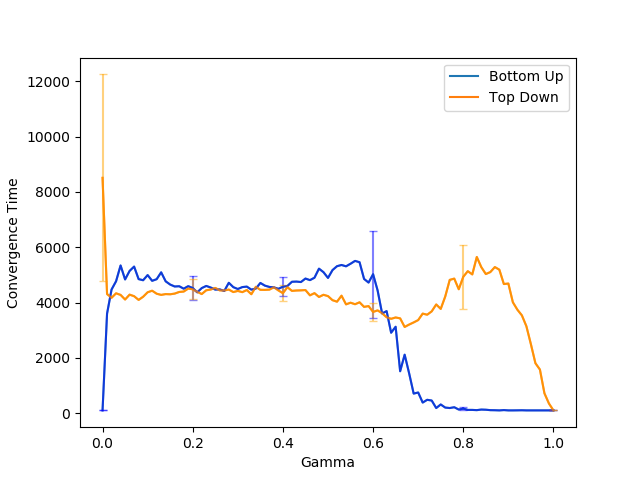
\includegraphics[width=\textwidth]{Images/Figures/BU+TD/FIE/Convergence_better.png}
    \caption{Convergence}
 \end{subfigure}
 \hfill
 \begin{subfigure}[ht]{0.45\textwidth}
    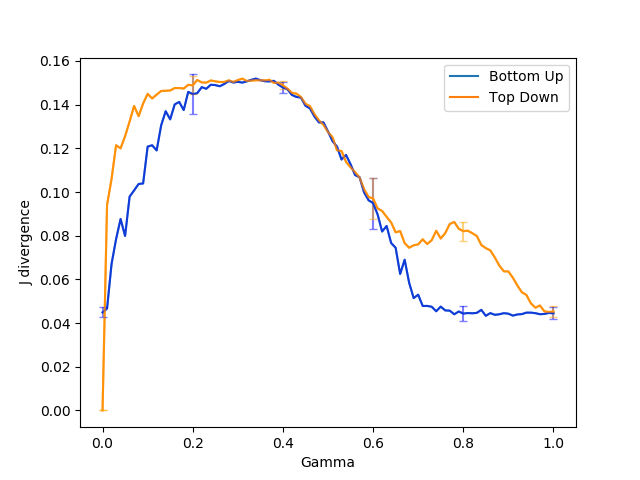
\includegraphics[width=\textwidth]{Images/Figures/BU+TD/FIE/J-Div_better.png}
    \caption{J-Divergence}
 \end{subfigure}
 %\hfill
 \begin{subfigure}[ht]{0.45\textwidth}
    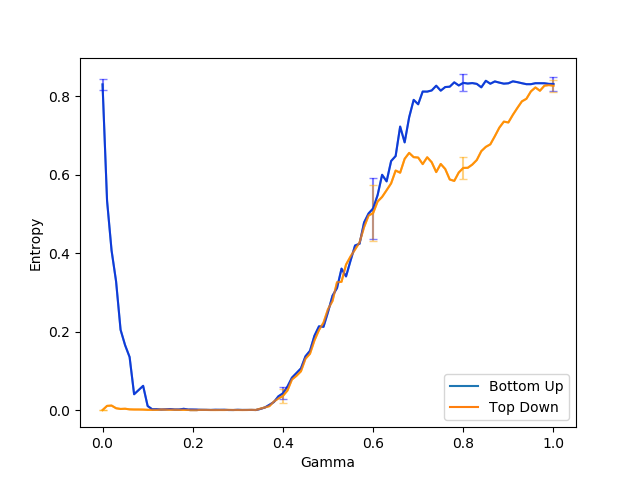
\includegraphics[width=\textwidth]{Images/Figures/BU+TD/FIE/Entropy_better.png}
    \caption{Entropy}
 \end{subfigure}

 \caption{Three plots showing the convergent behaviour of the Bottom Up and Top Down models with Discerning listeners as $\gamma$ is varied. (a) shows the time to convergence as defined by~\cref{eq:convergence}. (b) shows the average J-Divergence of the system at the corresponding iteration of (a). (c) shows the average entropy of the system at the corresponding iteration of (a). If the system has not converged within $50,000$ iterations, the point is left blank.} \label{fig:convergence_FIE}
\end{figure}



Here, the models converge at approximately the same rate for $ 0 \leq \gamma \leq 0.6$. However, it can be seen that the J-Divergence follows a parabola for this range of parameter values. This shows that the population is divided. As soon as the agents have the ability to ignore information their peers present, they form local consensuses. This manifests as groups of agents in different corners of the simplex, unable to accept an argument that comes from an agent in a different corner. As $\gamma$ increases, this division lessens, with agents becoming more able to hear other points of view. As $\gamma$ increases above $0.6$, the Bottom Up model begins to converge much more rapidly, as in the previous example. This is due to the harshness of the restriction placed on the speakers for high values of $\gamma$. As for high values of $\gamma$, the speaker must hold an extreme belief in a single state to be able to assert anything other than $\emptyset$. \Cref{fig:convergence_FIE} shows that both models converge at $4,000$ on average, significantly less than with Passive listeners. This is due to the local consensuses. The agents divide into small groups with low entropy values that change little over time, and so convergence is recorded without having to persuade the entire population to believe in a single state.  

The primary difference that emerges between these two models appears after $\gamma = 0.6$, where both entropy and J-Divergence plateau momentarily in the Top Down model. The difference is slight, and it is unclear exactly why it occurs. It is possible that this occurs because the Top Down model produces patterns such as those shown in~\cref{fig:sierpinski_triangle_intro}. The plateau indicates that these patterns are more stable than those formed by the Bottom Up model. At high values of $\gamma$, the Top Down model is likely to assert more general statements, and the listeners are more likely to accept them, leading to a more disparate and uncertain population than for the Bottom Up agents.

These results show that, when the listeners are capable of disregarding the assertions of a speaker, the population divides, forming local consensuses. Furthermore, the Top Down model is a slightly more robust solution for a wider range of $\gamma$. This is likely due to the greater level of flexibility built into the model. 



Now consider the convergence when the population comprised of Backfiring listeners. 


\begin{figure}
 \centering
  \begin{subfigure}[ht]{0.45\textwidth}
    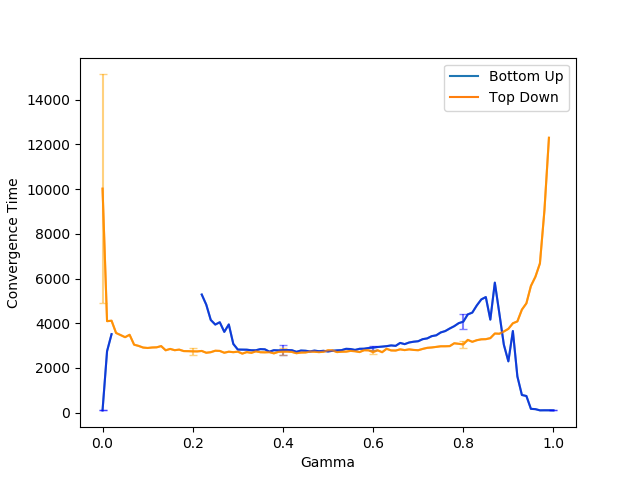
\includegraphics[width=\textwidth]{Images/Figures/BU+TD/Spiteful/Convergence.png}
    \caption{Convergence}
 \end{subfigure}
 \hfill
 \begin{subfigure}[ht]{0.45\textwidth}
    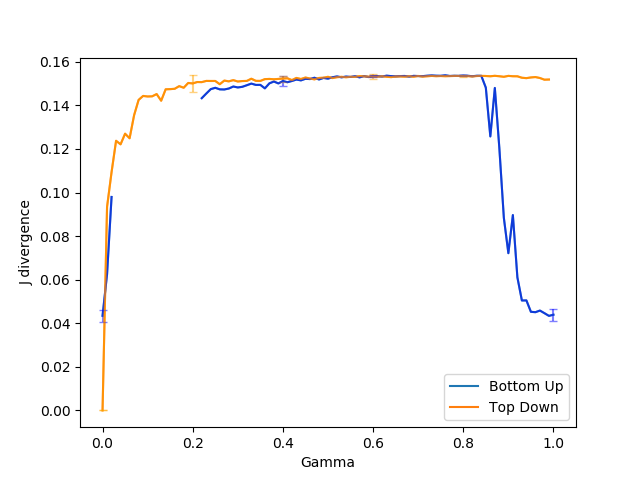
\includegraphics[width=\textwidth]{Images/Figures/BU+TD/Spiteful/J-Div.png}
    \caption{J-Divergence}
 \end{subfigure}
 \hfill
 \begin{subfigure}[ht]{0.45\textwidth}
    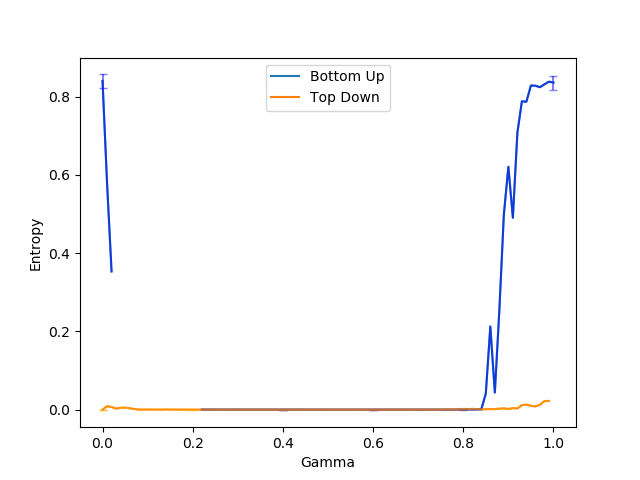
\includegraphics[width=\textwidth]{Images/Figures/BU+TD/Spiteful/Entropy.png}
    \caption{Entropy}
 \end{subfigure}
 \caption{Three plots showing the convergent behaviour of the Bottom Up and Top Down models with Backfiring listeners as $\gamma$ is varied. (a) shows the time to convergence as defined by~\cref{eq:convergence}. (b) shows the average J-Divergence of the system at the corresponding iteration of (a). (c) shows the average entropy of the system at the corresponding iteration of (a). If the system has not converged within $50,000$ iterations, the point is left blank.}\label{fig:convergence_Spite}
\end{figure}


It is clear from~\cref{fig:convergence_Spite} that the Bottom Up model fails to converge for $0.05 \leq \gamma \leq 0.2$. This is likely due to the general nature of a Bottom Up agent's assertions at these low values of $\gamma$. If the listener finds any one of the asserted states to be sufficiently improbable, they update on the complement of the asserted state, so general statements are less likely to meet this requirement than singletons.

It is apparent from the low value of entropy and high value of J-Divergence that the agents again reach local consensuses; they form distinct groups on the vertices of the simplex and are unable to listen to opposing arguments. Interestingly, the introduction of Backfiring listeners appears to have reduced the average convergence time compared to~\cref{fig:convergence_FIE} by $1,000$ iterations, a factor of $0.78$. This is likely due to the fact that, with Backfiring listeners, an agent updates at every iteration. The increased polarisation of updating on $\mathbf{A}^c$ will also contribute to an initial rapid division in the population. 


Finally, let us consider an Acclimatising population. Here, the population places less and less importance on new information as they receive each new argument. This promotes the stagnation of beliefs. \Cref{fig:convergence_Ageing} shows the convergence plots. 


\begin{figure}
 \centering
  \begin{subfigure}[ht]{0.45\textwidth}
    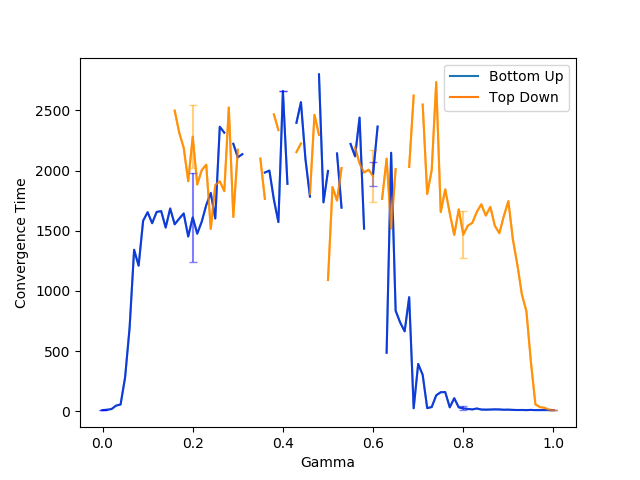
\includegraphics[width=\textwidth]{Images/Figures/ListenerModelPlots/Ageing/AgeingConvergenceDONTDELETE.png}
    \caption{Convergence}
 \end{subfigure}
 \hfill
 \begin{subfigure}[ht]{0.45\textwidth}
    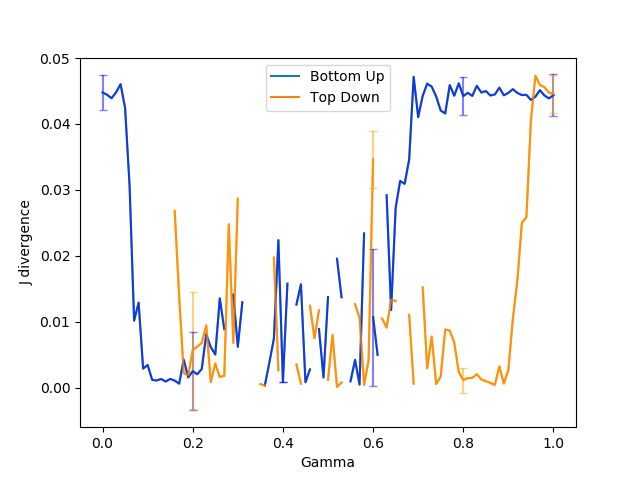
\includegraphics[width=\textwidth]{Images/Figures/ListenerModelPlots/Ageing/AgeingJ-DivDONTDELETE.png}
    \caption{J-Divergence}
 \end{subfigure}
 \hfill
 \begin{subfigure}[ht]{0.45\textwidth}
    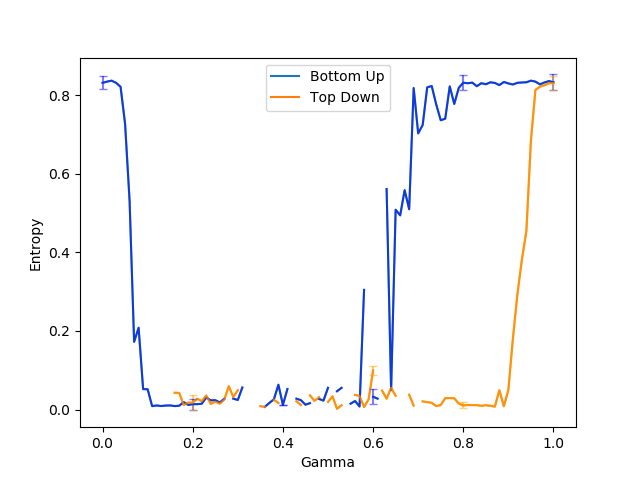
\includegraphics[width=\textwidth]{Images/Figures/ListenerModelPlots/Ageing/AgeingEntropyDONTDELETE(copy).png}
    \caption{Entropy}
 \end{subfigure}
 \caption{Three plots showing the convergent behaviour of the Bottom Up and Top Down models with Acclimatising listeners as $\gamma$ is varied. (a) shows the time to convergence as defined by~\cref{eq:convergence}. (b) shows the average J-Divergence of the system at the corresponding iteration of (a). (c) shows the average entropy of the system at the corresponding iteration of (a). If the system has not converged within $50,000$ iterations, the point is left blank.}\label{fig:convergence_Ageing}
\end{figure}


The results of these simulations are significantly more noisy than the other listener models. This is attributed to a number of factors. Firstly, this model converges within at most $2,500$ iterations, less than a third of the time taken by the Passive listener model, as one might expect. However, this rapid convergence both increases the appearance noise, by reducing the scale of the $y$-axis as well as increases the likelihood of variation in the results. When the simulation converges in so few iterations, minor anomalies in the order and nature of the arguments made in the population cause significant variation in the convergent behaviour of the system. For instance, consider an agent undecided between two possible states $H_1, H_2$, between which the remainder of the population is split evenly. If the individual agent repeatedly receives an argument in favour of $H_1$, it will update toward it, changing the entropy of the system. Whereas, if it receives alternating arguments, they will cancel out, registering as convergence. This leads to increased variation in the convergence times, dictated by the proportion of the population that is split between multiple states.

Despite this noise, observations can still be made. The convergence time under the Acclimatisation model is approximately one third less any other model, as one might expect. The agents update less and less upon hearing new information and so the rate of change in entropy decreases. For both speaker models, it can be seen that the entropy level is low for intermediate values of $\gamma$, with the Bottom Up model experiencing the same problem creating an argument is described in previous sections as $\gamma$ increases. The J-Divergence demonstrates a feature that has not previously been seen. While highly noisy, this plot shows that it is common to have non-zero J-Divergence using this model. Therefore, it must be the case that agents are spread out. However, in this model, this occurs in the following way. 

Consider a population with two local consensuses, where the population split approximately evenly between two states, as above. An agent that is undecided between the two will lie on the edge of the simplex. It will receive arguments from both subsets of the population, only increasing $\tau$, making the agent more stubborn. This agent will remain caught between the two groups until the system is said to have converged. The two main groups of agents will reinforce their current beliefs by communicating with other agents within the local consensus. This division in the population does not arise consistently, hence the noise in the J-Divergence plots. 


The Acclimatisation model shows similar behaviour for both the Bottom Up and Top Down models, both mostly achieving a population of agents certain in one state. However, this model occasionally divides the population. The main advantages of this model are the rapid convergence, and the ability for agents to grow wise with time. 





The results presented in this analysis demonstrate that when agents openly express the exact nature of their beliefs, the population becomes unanimously uncertain. However, when agents express arguments as sets of possible states of the world, it becomes possible for the population to form a global consensus in a single state, provided the listener agents are Passive. All the plots in this section demonstrate similarities between the Bottom Up and Top Down models for intermediate values of $\gamma$. However, for extremely high values, the Bottom Up model fails to produce meaningful assertions. The Top Down model is more robust, with slow convergence times occurring for very low values of $\gamma$. The two behave similarly, although Top Down model is a more robust approach for a wider range of values for $\gamma$. Furthermore, the Optimised model is shown to be incapable of reliably producing a consensus in a single state of the world, highlighting that its unconstrained approach is disadvantageous for the population. 

When listeners are able to discriminate, rejecting information that they deem unlikely, the population polarises. Local consensuses form, with subsets of the population unable to communicate with each other. This results in more rapid convergence, though not to a single state of the world. Finally, agents in the Acclimatising model converge more rapidly than any other model, though unpredictably lead to divisions in the population, again forming local consensuses. The only models that regularly give rise to global consensus in a single belief are the Top Down and Bottom Up models with Passive listeners, with the Top Down model behaving consistently across the full range of $\gamma$. 
